\chapter{Conceptual Model}
In the previous chapter, a general introduction to geothermal reservoir was given along with a brief understanding of scaling. 
In this chapter, a conceptual model for the geothermal reservoir will be discussed along with the boundary conditions set which will then be used to implement in PHREEQC. 

\section{Diagram}

In the Figure \ref{fig:conc}, the conceptual model has been designed.
\begin{figure}[h]
    \centering
    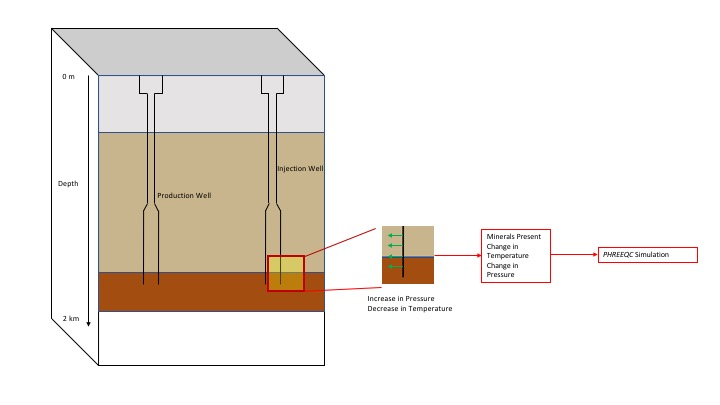
\includegraphics[scale=0.7]{ConcModel.jpg}
    \caption{Conceptual Model}
    \label{fig:conc}
\end{figure}
At the reservoir, the hot water present with certain chemical composition is available and is brought to the surface by the production well. When, the fluid reaches the surface it loses heat to heat exchangers. The change in temperature causes a change in the chemical composition of the fluid to change, which eventually leads into scaling of the pipe. Later, the fluid is then condensed and re-injected into the reservoir which again causes a change in the chemical composition which then leads to scaling. See Fig.  \ref{fig:conc}

In the figure, a macroscopic, meso-scropic and microscopic model has been structured. In the right side of the figure, i.e., the injection well there is an increase in the well pressure and a decline in the temperature. In the left side, the production well there is only decline in pressure.This chance in pressure or temperature as mentioned earlier leads to scaling and further change will lead to continuous scaling of the well or the pipe. 

Due to the scaling, there is then a change in the mineral composition of the fluid and hence we obtain a new pore fluid. In this paper, about saturation indices of 22 minerals are considered and modelled in PHREEQC. A list of these minerals with their chemical formula can be found in Appendix 1. Moreover, we are considering both the change in production well and the injection well along with considering re-injection in the doublet, 

To summarize the idea behind the conceptual model, it can be established that: 

In the mentioned model, the boundary condition is set up at the production well, the injection well and the condenser: 
\begin{table}[h!]
\centering
\begin{tabular}{|l|l|l|l|l|}
\hline
                 & Pressure (bar) & Temperature (Celsius) & Presence of Oxygen & Phase of Liquid                \\ \hline
Production Well  & 1 - 30        & 150 - 400             & No                 & Two phase or super saturated   \\ \hline
Reinjection Well &  20 - 300       & 50 - 150              & Possible           & Liquid or possible bubbles     \\ \hline
Condenser        & 0.08 - 0.12    & 25 - 35               & Yes                & Liquid Dissolved (CO$_2$ and H$_2$S) \\ \hline
\end{tabular}
\end{table}